\documentclass{article}
\usepackage{secdot}
\usepackage[utf8]{inputenc}
\usepackage[a4paper, portrait, margin=2.5cm]{geometry}
\usepackage{polski}
\usepackage{listings}
\usepackage{xcolor}
\usepackage{graphicx}
\usepackage{epstopdf}
\usepackage{float}
\usepackage{amsmath, amssymb, amsfonts}

\setlength\parindent{0pt}
\renewcommand{\arraystretch}{1.3}
\newcommand\norm[1]{\left\lVert#1\right\rVert}

\begin{document}

\lstset{basicstyle=\ttfamily\footnotesize, breaklines=true}
 \lstset{literate={ą}{{\k{a}}}1 {ł}{{\l{}}}1 {ń}{{\'n}}1 {ę}{{\k{e}}}1 {ś}{{\'s}}1 {ż}{{\.z}}1 {ó}{{\'o}}1 {ź}{{\'z}}1 {Ą}{{\k{A}}}1 {Ł}{{\L{}}}1 {Ń}{{\'N}}1 {Ę}{{\k{E}}}1 {Ś}{{\'S}}1 {Ż}{{\.Z}}1 {Ó}{{\'O}}1 {Ź}{{\'Z}}1 {ć}{{\'c}}1 {Ć}{{\'C}}1 }
\definecolor{bgcolor}{rgb}{0.95,0.95,0.95}
\lstset{
    backgroundcolor=\color{bgcolor},
    framexleftmargin=0.5cm,
    framexrightmargin=0.5cm,
    framextopmargin=0.3cm,
    framexbottommargin=0.3cm, 
    aboveskip=1em,
    belowskip=1em,
    frame=tb, framerule=0pt,
}
 
\begin{center}
  \Huge
  \textbf{Zadanie labolatoryjne z Matematyki Obliczeniowej} \\[0.5cm]
  
  \large
  Krzysztof Antoniak 358985
\end{center}

\section{Zawartość projektu}
Archiwum zawiera pliki \verb|ROZKLAD.m| oraz \verb|ROZWIAZ.m| implementujące funkcje z polecenia.

\lstinputlisting[language=Octave]{rozklad_help.m}
\lstinputlisting[language=Octave]{rozwiaz_help.m}

Algorytmy zostały zaimplementowane na podstawie skryptu "Trzynaście Wykładów z Matematyki Obliczeniowej" oraz materiałów z Ważniaka, z drobnymi zmianami przy pełnym wyborze elementu głównego.

\section{Testy}
Projekt zawiera zestaw testów sprawdzających poprawność i czas wykonania algorytmów dla różnych klas macierzy.

Testy zostały przeprowadzone w Octave (GUI) 4.2.1 dla Windows na 64-bitowym procesorze o taktowaniu 2.80 GHz. \texttt{eps = 2.2204e-016}.

\subsection{\texttt{test\_zero\_on\_diagonal.m}}
Test sprawdza działanie rozkładu w przypadku wystąpienia zera na przekątnej w macierzy wejściowej. W przypadku rozkładu bez wyboru elementu głównego funkcja \verb|ROZKLAD| powinna zwrócić błąd.
\lstinputlisting[language=Octave]{test_zero_on_diagonal.m}

\subsection{\texttt{test\_error\_random\_matrices.m}}
Test porównuje błąd względny rozwiązania układu równań. Układy są reprezentowane przez losowe macierze, przy rosnącym wymiarze macierzy.

\begin{figure}[H]
    \centering
    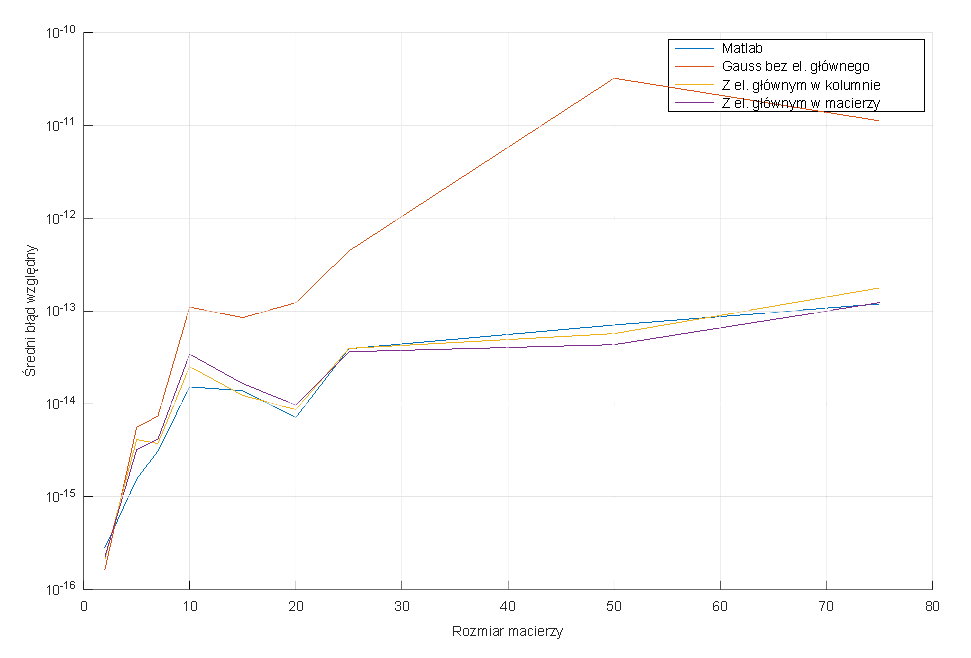
\includegraphics[scale=1]{test_error_random_matrices}
    \caption{Porównanie średnich błędów względnych rozwiązania układu równań dla losowych macierzy}
\end{figure}

\begin{table}[H]
    \centering
    \begin{tabular}{ |c|r|r|r|r| }
        \hline
        Rozmiar macierzy & Octave & \verb|ROZKLAD(A, 0)| & \verb|ROZKLAD(A, 1)| & \verb|ROZKLAD(A, 2)| \\
        \hline
         2 & 2.8198e-016 & 1.6246e-016 & 2.1306e-016 & 2.2392e-016 \\
         5 & 1.5445e-015 & 5.5954e-015 & 4.1216e-015 & 3.2173e-015 \\
         7 & 3.1045e-015 & 7.3689e-015 & 3.7419e-015 & 4.1710e-015 \\
        10 & 1.5264e-014 & 1.1022e-013 & 2.5273e-014 & 3.4381e-014 \\
        15 & 1.3864e-014 & 8.5201e-014 & 1.2323e-014 & 1.6534e-014 \\
        20 & 7.1319e-015 & 1.2287e-013 & 8.6905e-015 & 9.6939e-015 \\
        25 & 3.9295e-014 & 4.4389e-013 & 3.9567e-014 & 3.6472e-014 \\
        50 & 7.0803e-014 & 3.2336e-011 & 5.7115e-014 & 4.3483e-014 \\
        75 & 1.1944e-013 & 1.1238e-011 & 1.7718e-013 & 1.2301e-013 \\
        \hline
    \end{tabular}
    \caption{Porównanie średnich błędów względnych rozwiązania układu równań dla losowych macierzy}
\end{table}

Eliminacja Gaussa wypada w teście bardzo słabo, błąd rośnie bardzo szybko. W przypadku pozostałych metod błąd rośnie mniej więcej w tym samym tempie. Wniosek: lepsza strategia pivotingu nie poprawia znacząco dokładności. Co ciekawe, błąd według implementacji Octave jest zaczyna być niższy dopiero dla macierzy rozmiaru większego niż 50.

\subsection{\texttt{test\_error\_hilbert\_matrices.m}}
Test porównuje błąd względny rozwiązania układu równań. Układy są reprezentowane przez macierz Hilberta o rosnącym rozmiarze.

\begin{figure}[H]
    \centering
    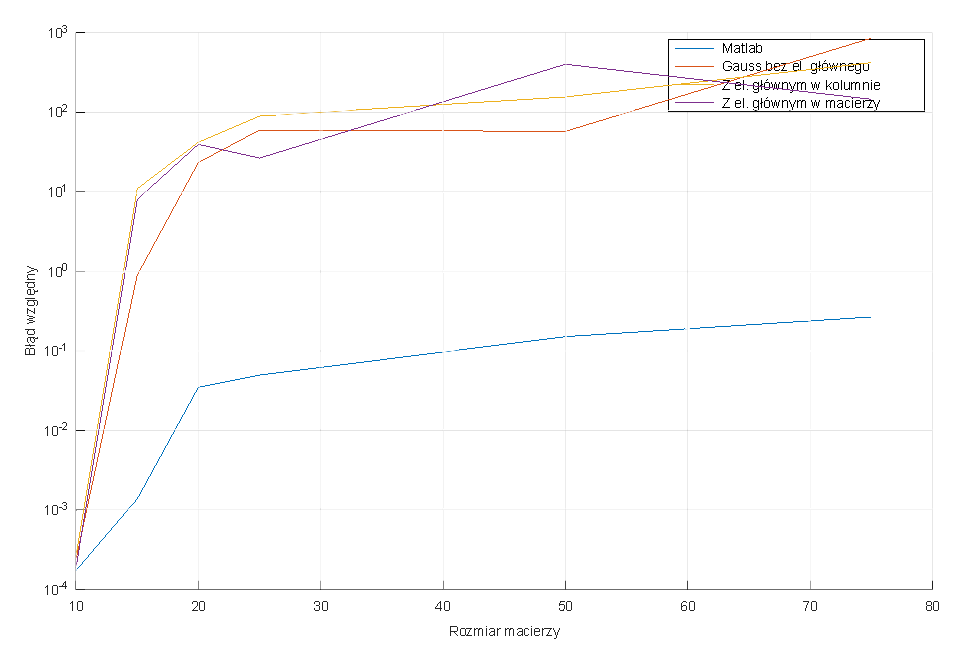
\includegraphics[scale=1]{test_error_hilbert_matrices}
    \caption{Porównanie błędów względnych rozwiązania układu równań danego macierzą Hilberta}
\end{figure}

\begin{table}[H]
    \centering
    \begin{tabular}{ |c|r|r|r|r|r| }
        \hline
        Rozmiar & \verb|cond(hilb(N))| & Octave & \verb|ROZKLAD(A, 0)| & \verb|ROZKLAD(A, 1)| & \verb|ROZKLAD(A, 2)| \\
        \hline
        10 & 1.6024e+013 & 0.00017291 & 0.00023976 & 0.00026789 & 0.00018998 \\
        15 & 3.6744e+017 & 0.0013725 & 0.8901 & 10.874 & 7.9896 \\
        20 & 1.3554e+018 & 0.03468 & 23.296 & 41.943 & 39.396 \\
        25 & 1.3719e+018 & 0.049536 & 59.561 & 89.531 & 26.484 \\
        50 & 2.3125e+019 & 0.15065 & 57.445 & 155.82 & 401.55 \\
        75 & 8.2694e+018 & 0.26706 & 852.04 & 419.62 & 145.47 \\
        \hline
    \end{tabular}
    \caption{Porównanie błędów względnych rozwiązania układu równań danego macierzą Hilberta}
\end{table}

Macierze Hilberta są bardzo źle uwarunkowane, więc numeryczna dokładność obliczeń jest bardzo niska i błyskawicznie spada wraz ze wzrostem rozmiaru macierzy. Już przy rozmiarze 15x15 błąd względny ma rząd wielkości 1.

\subsection{\texttt{test\_error\_matrix1\_matrices.m}}
Test porównuje błąd względny rozwiązania układu równań, który jest dany specjalną macierzą o następującym formacie:

\lstinputlisting[language=Octave]{matrix1.m}

\begin{figure}[H]
    \centering
    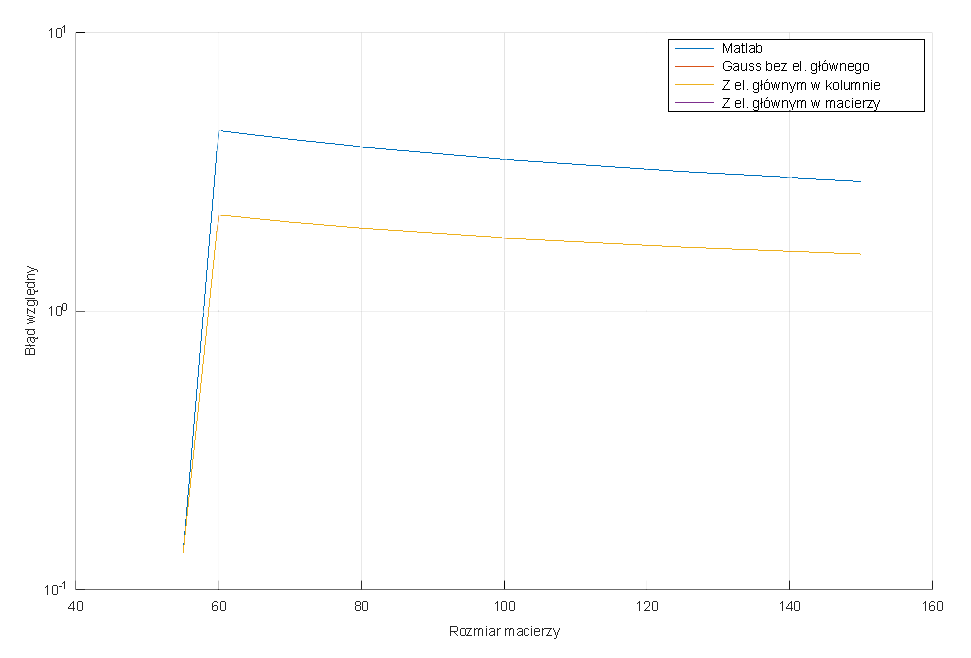
\includegraphics[scale=1]{test_error_matrix1_matrices}
    \caption{Porównanie błędów względnych rozwiązania układu równań danego macierzą "jedynkową"}
\end{figure}

\begin{table}[H]
    \centering
    \begin{tabular}{ |c|r|r|r|r| }
        \hline
        Rozmiar & Octave & \verb|ROZKLAD(A, 0)| & \verb|ROZKLAD(A, 1)| & \verb|ROZKLAD(A, 2)| \\
        \hline
        50 & 0 & 0 & 0 & 0 \\
        54 & 0 & 0 & 0 & 0 \\
        55 & 0.13484 & 0.13484 & 0.13484 & 0 \\
        60 & 4.45350 & 2.21860 & 2.21860 & 0 \\
        70 & 4.14040 & 2.08850 & 2.08850 & 0 \\
        80 & 3.88910 & 1.98540 & 1.98540 & 0 \\
        100 & 3.50710 & 1.83120 & 1.83120 & 0 \\
        125 & 3.16860 & 1.69780 & 1.69780 & 0 \\
        150 & 2.92120 & 1.60280 & 1.60280 & 0 \\
        \hline
    \end{tabular}
    \caption{Porównanie błędów względnych rozwiązania układu równań danego macierzą "jedynkową"}
\end{table}

Tutaj problemem jest reprezentacja liczb całkowitych. Ogólnie wiemy, że zachodzi $ \norm{x - fl_\nu(x)} \lessapprox K(n)\nu \cdot cond(A) \cdot \norm{x} $. Akurat w tym przypadku $ K(n) \approx 2^n $, a jednocześnie $ \nu \approx 10^-16 \approx 2^-55 $. Stąd błędy przy więcej niż 54 wierszach. Liczby całkowite w Octave są traktowane jak rzeczywiste. Powyżej pewnej wartości ich końcówka zostaje zaookrąglona i to powoduje błąd.

W przypadku wyboru elementu głównego w podmacierzy nie występuje żaden błąd. W trakcie wykonania ostatnia kolumna zostaje wstawiona między pierwszą i drugą.

\subsection{\texttt{test\_time\_random\_matrices\_vs\_matlab.m}}
Test sprawdza średni czas rozkładu dla macierzy losowych. Testowane są zaimplementowane warianty rozkładu przy rosnącym wymiarze macierzy.

\begin{figure}[H]
    \centering
    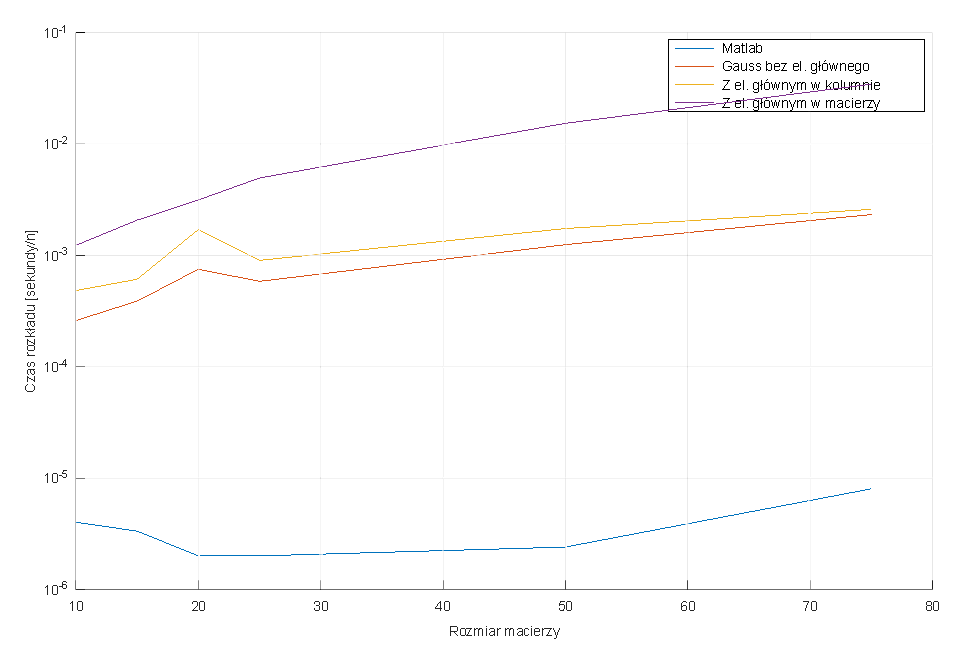
\includegraphics[scale=1]{test_time_random_matrices_vs_matlab}
    \caption{Porównanie średnich czasów rozkładu macierzy (sekundy/n)}
\end{figure}

\begin{table}[H]
    \centering
    \begin{tabular}{ |c|r|r|r|r| }
        \hline
        Rozmiar & \verb|lu(A)| & \verb|ROZKLAD(A, 0)| & \verb|ROZKLAD(A, 1)| & \verb|ROZKLAD(A, 2)| \\
        \hline
        10 & 4.0078e-006 & 0.00026018 & 0.00048338 & 0.0012329 \\
        15 & 3.3401e-006 & 0.00038827 & 0.00061045 & 0.0020755 \\
        20 & 2.0010e-006 & 0.00075103 & 0.00170620 & 0.0031438 \\
        25 & 2.0008e-006 & 0.00058441 & 0.00090144 & 0.0049543 \\
        50 & 2.4004e-006 & 0.00124930 & 0.00174210 & 0.0153550 \\
        75 & 8.0058e-006 & 0.00232650 & 0.00259080 & 0.0345240 \\
        \hline
    \end{tabular}
    \caption{Porównanie średnich czasów rozkładu macierzy (sekundy/n)}
\end{table}

Czas wykonania w wariancie z el. głównym w kolumnie nie jest znacząco większy. Koszt obliczeń wzrasta dużo szybciej w wariancie z wyborem elementu głównego w całej podmacierzy. Wynika to stąd, że skrypt musi wykonać porównania dla $n^2$ pól macierzy.

Z poprzednich testów wynika, że wybór elementu głównego w podmacierzy nie poprawia znacząco wyniku. Jednocześnie jest on dość kosztowny czasowo.

\end{document}
